\documentclass[]{politex}
% ========== Opções ==========
% pnumromarab - Numeração de páginas usando algarismos romanos na parte pré-textual e arábicos na parte textual
% abnttoc - Forçar paginação no sumário conforme ABNT (inclui "p." na frente das páginas)
% normalnum - Numeração contínua de figuras e tabelas 
%	(caso contrário, a numeração é reiniciada a cada capítulo)
% draftprint - Ajusta as margens para impressão de rascunhos
%	(reduz a margem interna)
% twosideprint - Ajusta as margens para impressão frente e verso
% capsec - Forçar letras maiúsculas no título das seções
% espacosimples - Documento usando espaçamento simples
% espacoduplo - Documento usando espaçamento duplo
%	(o padrão é usar espaçamento 1.5)
% times - Tenta usar a fonte Times New Roman para o corpo do texto
% noindentfirst - Não indenta o primeiro parágrafo dos capítulos/seções


% ========== Packages ==========
\usepackage[utf8]{inputenc}
\usepackage{amsmath,amsthm,amsfonts,amssymb}
\usepackage{graphicx,cite,enumerate}
\usepackage{makecell}
\graphicspath{ {./images/} }
\usepackage{placeins}
\usepackage{enumitem}


% ========== Language options ==========
\usepackage[brazil]{babel}
%\usepackage[english]{babel}


% ========== ABNT (requer ABNTeX 2) ==========
%	http://www.ctan.org/tex-archive/macros/latex/contrib/abntex2
\usepackage[num]{abntex2cite}

% Forçar o abntex2 a usar [ ] nas referências ao invés de ( )
\citebrackets{[}{]}


% ========== Lorem ipsum ==========
\usepackage{blindtext}



% ========== Opções do documento ==========
% Título
\titulo{SIMIOS - Sistema de Monitoramento de Interação Orgânica entre Símios}

% Autor
\autor{Larissa Mangolim Amaral \\%
		Luciana da Costa Marques \\%
		Pedro Orscar Gallo Vaz}

% Para múltiplos autores (TCC)
%\autor{Nome Sobrenome\\%
%		Nome Sobrenome\\%
%		Nome Sobrenome}

% Orientador / Coorientador
\orientador{Professor Livre-Docente Carlos Eduardo Cugnasca}
\coorientador{Professor Doutor Bruno de Carvalho Albertini}

% Tipo de documento
\tcc{Eletricista com ênfase em Computação}
%\dissertacao{Engenharia Elétrica}
%\teseDOC{Engenharia Elétrica}
%\teseLD
%\memorialLD

% Departamento e área de concentração
%\departamento{Nome do departamento}
%\areaConcentracao{Área de concentração}

% Local
\local{São Paulo}

% Ano
\data{2018}




\begin{document}
% ========== Capa e folhas de rosto ==========
\capa
\falsafolhaderosto
\folhaderosto


% ========== Folha de assinaturas (opcional) ==========
\begin{folhadeaprovacao}
	\assinatura{Prof.\ Livre-Docente Carlos Eduardo Cugnasca}
%	\assinatura{Prof.\ Y}
%	\assinatura{Prof.\ Z}
\end{folhadeaprovacao}


% ========== Ficha catalográfica ==========
% Fazer solicitação no site:
%	http://www.poli.usp.br/en/bibliotecas/servicos/catalogacao-na-publicacao.html


% ========== Dedicatória (opcional) ==========
%\dedicatoria{Dedicatória}


% ========== Agradecimentos ==========
\begin{agradecimentos}
Às nossas famílias e amigos, por todo o apoio, suporte e carinho imensuráveis.

Aos professores orientadores, agradecemos a dedicação para o auxílio intelectual e encaminhamento deste trabalho.

À Professora Doutora Cristiane Schilbach Pizzutto, por sua saborosa contribuição para nossa compreensão da óptica do cientista veterinário.

Ao professor Reginaldo Arakaki, por ter disponibilizado os recursos e orientações iniciais e com isso ter permitido os primeiros passos do projeto.

À professora Lúcia Filgueiras, por ter dado uma visão multidisciplinar do que se poderia fazer no aprimoramento da Interface Humano-Computador e pelo incentivo e ajuda na determinação do domínio do problema.

Ao professor Jorge Kinoshita, pelo apoio semanal na operação com Sistemas Embarcados, pelas críticas construtivas e preocupação sincera com o sucesso do trabalho.

Ao pós-doutorando Wilian França Costa, pela orientação para a familiarização das ferramentas do projeto durante todo o período de sua elaboração.

Aos demais professores e colegas que contribuíram através de nossa formação como engenheiros e como pessoas.
\end{agradecimentos}


% ========== Epígrafe (opcional) ==========
%\epigrafe{%
%	\emph{``Epígrafe''}
%	\begin{flushright}
%		-{}- Autor
%	\end{flushright}
%}


% ========== Resumo ==========
\begin{resumo}
A execução deste trabalho visa a projeção e implementação de um sistema capaz de auxiliar pesquisadores de saúde e biologia animal no monitoramento comportamental de uma população em estudo. Para tal, foi elaborado um wearable capaz de obter a localização de animais em observação inseridos em ambiente controlado no qual uma rede de sensores é integrada. Tal informação é enviada para uma plataforma onde os dados poderão ser analisados pelo pesquisador remotamente. O desenvolvimento deste sistema tem como finalidade atender às necessidades de monitoramento de símios na reserva natural do Instituto Butantã da Universidade de São Paulo. Contudo, pretende-se que sua aplicação seja possível em distintas reservas, para a observação de diferentes animais e que possa eventualmente ser expandido para captar demais variáveis de controle relevantes para o biólogo ou veterinário. Finalmente, o sistema obtido cumpre os requisitos definidos e demonstra escalabilidade.

\textbf{Palavras-Chave} -- Monitoramento animal remoto, Redes de sensores sem fio, Embarcado.
\end{resumo}


% ========== Abstract ==========
\begin{abstract}
This study presents the design and implementation of an entire system capable of assisting animal health and biology researchers monitoring the object of study. Therefore, an embedded wearable was programmed so that the system could provide the researcher remotely with the observed animals’ location. For that to happen, they would have to be living in a natural reserve mapped by a wireless sensor network. This system’s purpose is to meet Instituto Butantã’s needs regarding monitoring apes inside the reserve. However, it is expected that this system is also applicable inside many different reserves, for distinct mammals observation and open to be expanded so that it shall be able to monitor as many other control variables the biologist or veterinary finds relevant. The final work meets the defined requirements and shows scalability.

\textbf{Keywords} -- Remote animal monitoring, Wireless sensor network, Embedded.
\end{abstract}


% ========== Listas (opcional) ==========
\listadefiguras
\listadetabelas

% ========== Listas definidas pelo usuário (opcional) ==========
\begin{pretextualsection}{Lista de abreviaturas e siglas}

GPS \textit{Global Positioning System}

MVC \textit{Model-view-controller}

RFID \textit{Radio-Frequency Identification}

RSSI \textit{Received Signal Strength Indication}

TI \textit{Texas Instruments}

\end{pretextualsection}

% ========== Sumário ==========
\sumario



% ========== Elementos textuais ==========

%\chapter{Introdução}
Neste capítulo, será explicado o escopo do trabalho - o que vai ser projetado -, quais resultados esperamos obter e por que o fazemos.

\section{Objetivo}
Este trabalho visa o projeto e implementação da base de um sistema capaz de obter e apresentar a localização de animais, dando abertura para que possa ser expandido e que sua complexidade possa ser refinada a ponto de ser aplicável em reservas naturais, chegando a capturar inclusive outros dados de interesse acadêmico.

Está dentro do escopo deste projeto: a escolha das informações sendo colhidas dos animais; o método pelo qual elas são obtidas, calculadas ou inferidas; a maneira como elas são transmitidas, armazenadas e apresentadas; a escolha e implementação das tecnologias utilizadas; e a avaliação de desempenho sobre sua operação.

A composição do sistema prevê que dispositivos embarcados inseridos em mochilas anexadas ao macaco possam ser mapeados por uma rede de sensores introduzida nas árvores do ambiente natural. Dispositivos centrais de comunicação também inseridos no ambiente realizarão a coleta dessas informações, a fim de enviá-las para retenção em um servidor. Este realiza o processamento e armazenamento dos dados que são injetados em uma interface em \emph{software} disponível para o usuário.

A discriminação do sistema é melhor realizada nos capítulos 4 e 6.

\section{Motivação}
Este trabalho visa atender às necessidade de monitoramento de símios nas reservas do Instituto Butantã da Universidade de São Paulo. Dentre elas, destaca-se: a coleta de informações sobre os animais de forma simples e sem viés, tais como suas disposições em bando e suas temperaturas corporais; e a apresentação destas, de forma a facilitar análise de dados em  pesquisas acadêmicas e a manutenção da saúde dos animais.

Além disso, propõe-se que o este trabalho possa ser aplicado em qualquer reserva que necessite monitorar o comportamento de um bando de animais, sendo para tanto, veemente generalizado neste documento.

Ao final, espera-se obter um sistema que cubra o funcionamento mínimo de requisitos funcionais especificados no capítulo 4.

\section{Justificativa}
Animais silvestres são difíceis de serem observados em habitat natural por uma série de motivos. Primeiro, a partir do momento que o pesquisador se coloca no campo de visão do animal para observá-lo gera viés no comportamento deste, pois o animal também detecta a presença daquele e em muitas instâncias, age de forma irregular. Um caso específico se encontra no contexto de desamamentação de filhotes de macacos, cuja prática é realizada exclusivamente em um ambiente recluso e onde a presença de outrem é inadmissível, portanto o conhecimento sobre este comportamento é limitado para os pesquisadores.

Segundo, o auxílio tecnológico para essa tarefa é complicado uma vez que as tecnologias mais comumente usadas para monitoramento (câmeras de vídeo)  e rastreamento (\emph{Global Positioning System} - GPS) são descartadas pela densidade da mata, que dificulta a observação, e imprecisão da informação obtida, que impede a inferência de comportamentos, respectivamente. Isso evidencia a necessidade de novas tecnologias a fim de automatizar os processos de pesquisa laboratorial e controle de localização de animais silvestres, tanto para o estudo sobre seu comportamento como para a manutenção de sua saúde.

Primordialmente, o conceito que move este projeto está atrelado ao que foi tratado por Handcock (2009) \cite{handcock} de que a interação social biológica revela preferências sociais e comportamentais. Por exemplo, é citado como o mapeamento de encontros entre machos e fêmeas pode correlacionar com acasalamento, o que possibilita estudos de emancipação genética em uma população.

Corolariamente, permeia o projeto o conceito de Saúde Única (One Health) abordado por Zinsstag (2011) \cite{zinsstag}, onde indissocia-se a visão de saúde humana, animal e do ambiente. Como do ponto de vista biológico o estudo do comportamento animal permite novas conclusões sobre seu comportamento em reservas e cativeiro, e sob o ponto de vista veterinário a análise dos dados sobre o animal e seu ambiente leva a melhoras na manutenção da saúde deste e do ambiente, sob ambos vê-se um impacto na saúde do homem. O sistema pode, por exemplo, ajudar na prevenção de febre amarela, por meio de coleta de dados em populações de animais alvos da doença.

\section{Organização do Trabalho}
O capítulo 2 deste trabalho relata os estudos realizados sobre conceitos fenotípicos e comportamentais do grupo de foco, sobre o contexto de pesquisa destes animais e sobre tecnologias voltadas para redes de sensores biológicos potencialmente válidas para este projeto.

O capítulo 3 trata da forma como o planejamento do sistema deverá ser pensado, enfatizando aspectos de projeto de sistemas embarcados.

No capítulo 4 são indicados os requisitos funcionais e não funcionais levantados e algumas das possíveis soluções para essas problemáticas.

O capítulo 5 destrincha as tecnologias de fato selecionadas para serem utilizadas no sistema a ser implementado, considerando seus pontos falhos mas acentuando o motivo de terem sido escolhidas.

O capítulo 6, por sua vez, trabalha de fato a projeção do sistema seguindo todos os princípios estudados nos capítulos anteriores para que esteja clara a maneira de implementá-lo. Neste mesmo capítulo, os aspectos que tocam a implementação do sistema, que consideram a parte prática do objeto de estudo, também são descritos.

Por fim, no capítulo 7 são mostrados os resultados obtidos a partir do sistema desenvolvido através de validações e testes quantitativos e qualitativos de desempenho e satisfação.


\chapter{Aspectos Conceituais}
Alguns dos principais conceitos para compreensão e contextualização deste projeto são trabalhados neste capítulo.

\section{Macacos e Reservas Naturais}
Para melhor compreensão do aspecto biológico que este trabalho toca, foi realizada uma entrevista com a professora Cristiane Pizzutto, que pode ser vista na íntegra no apêndice A deste documento.

A partir desta, foi possível quantificar alguns parâmetros importantes para o dimensionamento do projeto, tal como a quantidade comumente observada de animais em bandos de reservas e cativeiros, para qual foi assegurado que, considerando um bando de dez macacos, estaríamos abrangendo seguramente o suficiente.

Também foi possível notar como a tarefa de observação para aquisição de dados relativos aos animais, tais como sinais vitais, movimentação e alimentação, é exaustiva, toma tempo e pode ser objetiva o bastante para que possa ser realizada por um sistema remoto.

A parte subjetiva do levantamento de dados está relacionada às atividades e interações dos animais, que normalmente só podem ser adquiridos por observação direta. Essa é a parte que nosso projeto tenta abordar e que nos fez perceber que talvez, para cativeiro, o auxílio de câmeras com alguma inteligência seria bem vindo.

Outra questão levantada é de como estes dados são digeridos. A pesquisadora aponta que a manipulação dos dados é manual e que utilizam planilhas para obter estatísticas. Considerando a quantidade massiva de dados, seria interessante pensar em injetar conceitos de \emph{Big Data}.

\section{Tecnologias Potenciais}
\textbf{Redes de Sensores Sem Fio}

A emergência da tecnologia de Redes de Sensores Sem Fio (RSSF) permitiu não somente o monitoramento das variáveis de um objeto, mas também o supervisionamento de todo o contexto em que ele está incluído e da interação dele com os demais pontos do sistema sendo sensoriados.

RSSFs são especialmente relevantes quando se tratando de ambientes cuja área que deve ser coberta é muito extensa. Estas redes são compostas por nós interligados, em que cada nó deve ter sensores, processamento, memória, antena e bateria independentes e sustentáveis.

Dada essa composição, as RSSFs são capazes de satisfazer áreas de cobertura muito extensas e são ótimas para criar integração entre elementos que estão, localmente, constantemente conjuntos.

Por isso, compõem uma tecnologia ótima para organizações biológicas, que envolvem grandes populações distribuídas, sendo, portanto, frequentemente aplicadas em sistemas agrícolas.

Como enfatizado por Handcock (2009) \cite{handcock}, para animais essa utilidade também é incluída, mas prevê algumas ressalvas. Uma delas considera a situação de que o animal de vida livre pode permanecer por semanas fora do alcance de pontos de acesso que recebam seus dados e, por esse motivo, cada nó da rede deverá possuir bateria e memória suficientemente robustas. Para reduzir o tempo de ausência de resposta de um determinado indivíduo, é possível implementar escuta nos próprios nós da rede, de forma que os animais que entrarem em contato entre si mantenham as informações dos demais, aumentando a chance de que algum deles possa transmiti-las para o servidor no alcance de pontos de acesso. Essa prática, no entanto, exige ainda mais energia e armazenamento.

RSSFs são, por vezes, estudadas para posicionamento em ambientes internos, principalmente atreladas ao uso de pontos de acesso \emph{Wi-fi}, que já são naturalmente alocados nesses espaços para uso de internet.

\textbf{Rádio}
A aplicação tecnológica para rastreamento de animais mostra-se insistente no uso de transmissores de rádio por muitos anos, por mais que a tecnologia de localização para aplicações humanas já o tenha superado de longe.

O RFID (\emph{Radio Frequency Identification}) foi bastante usado para obter informações relacionadas à condição do animal identificado. Recentemente, estes transmissores têm sido também utilizados para detectar encontros sociais entre animais através de picos de intensidade do sinal de rádio sendo transmitido.

\textbf{GPS}
A emancipação do GPS aplicado ao smartphone praticamente trivializou a tarefa de localização, principalmente quando associada à mobilidade e roteamento.

A integração de tal tecnologia em sistemas biológicos demonstra uma tentativa de integrar o sensoriamento da interação do animal com o ambiente, como é salientado por Handcock \cite{handcock}.

O GPS, no entanto, tem uma série de complicações. Primeiramente, sua precisão em baixa escala é bem complicada. Handcock afirma que para obter boa acurácia, é necessário ter uma taxa de amostragem relativamente alta, o que é bastante ruim para a sustentabilidade da memória e da energia do sistema.

Um outro problema está relacionado à pouca praticidade do módulo GPS, que apresenta peso relativamente elevado (aproximadamente 10g) dependendo do animal que está sendo rastreado.

\section{Modelos Comerciais}
Alguns modelos de coleiras voltadas a mamíferos são citadas na tabela a seguir. Os produtos são fornecidos pela empresa ATS (\emph{Animal Traceability Solutions}) \cite{ats} que, infelizmente, não discrimina o porte recomendado do animal usuário em seu site, portanto só foi possível inferir o peso que o dispositivo deste projeto deveria ter confirmando o que havia sido relatado pelos pesquisadores: de algo de no máximo 10g, uma vez que macacos menores pesam cerca de 400g.

Por outro lado, foi possível conceber alguns potenciais modelos para o invólucro do produto final deste projeto, principalmente no que diz respeito ao material utilizado.

\begin{table}[ht]
\centering
\caption{Exemplos comerciais de coleiras de rastreamento de mamíferos da ATS}
\vspace{0.5cm}
\begin{tabular}{l|ccc}
\hline
Nome & \makecell{SM17X0 Mammal \\ Collar, X-Small} & \makecell{M15X5 Mammal \\ Zip-Tie Collar} & \makecell{W500 Wildlink GPS \\ Logger, Small Collar} \\

Imagem & \makecell{\includegraphics[scale=0.5]{ATS1}} & \makecell{\includegraphics[scale=0.5]{ATS2}} & \makecell{\includegraphics[scale=0.5]{ATS3}}\\% \vspace{0.4cm}\\

Peso & 9 a 16g & 10 a 40g & 65 a 115g\\ %\vspace{0.4cm}\\

Bateria & Lítio / 156 a 282 dias & Lítio / 195 a 596 dias & AA / 1,75 a 3,5 anos \\%\vspace{0.4cm} \\

Material &
\makecell{- Coleira de \\ \textbf{neoprene} \\
- Encapsulamento \\ de resina a prova \\ de água} &
\makecell{ - Coleira de \textbf{tubo} \\ \textbf{de plástico (cable-tie)} \\
- Encapsulamento \\ de resina a prova \\ de água} &
\makecell{- Coleira de \textbf{neoprene} \\ \textbf{ou nylon} }
\end{tabular}
\end{table}

Como visto no item anterior, comercialmente é utilizado rádio na maior parte dos casos (M17X0 e M15X5) e, eventualmente, GPS (W500 - para o qual é possível notar que exige um peso bem superior ao limite estabelecido de cerca de 10g).
\FloatBarrier

\section{Algoritmos}
Inicialmente, é necessário compreender uma forma de calcular a posição dos animais através da distância entre macaco e ponto de acesso. De praxe, em RSSFs este cálculo pode ser feito de duas formas.

A primeira delas é utilizando a intensidade do sinal (\emph{Received Signal Strength Indication} - RSSI). O cálculo da distância, neste caso, é dado pelo seguinte modelo proposto pela \emph{Texas Instruments} (TI), que é melhor detalhado por Dong e Dargie (2012) \cite{dong}.

\begin{equation}
RSSI = -10 \times n \times \log_{10} d + A
\end{equation}

Sendo:
\begin{itemize}
\item d a distância em metros
\item RSSI a intensidade do sinal em dBm
\item n a constante de propagação do sinal
\item A a intensidade do sinal para 1 metro de distância
\end{itemize}

Essa é uma maneira simples de baixo custo de implementação, porém, como é bem destacado por Larsson (2015) \cite{larsson}, dada a alta variação de n devido a suscetibilidade do sinal à interferência do meio, demonstra-se um tanto imprecisa.

A constante de propagação pode ser determinada empiricamente. Se sabe n=2 para o vácuo; no ar, valores coerentes estão entre 2.7 e 4. A determinação da constante para este projeto pode ser observada no apêndice.

Outra forma seria calcular a distância sabendo a velocidade de propagação do sinal no meio, dado o tempo que demora para que o sinal seja recebido a partir da implementação de um eco. Idealmente esta é uma abordagem muito mais precisa, que só é impossibilitada em casos que o hardware utilizado não possua relógio. No entanto, qualquer deficiência na temporização e sincronização, por menor que seja, pode comprometer a precisão de tal metodologia.

Para este projeto, pretende-se implementar a primeira forma e verificar a precisão da mesma.

Além disso, foi requerido desenvolver um algoritmo para obtenção do mapeamento da posição dos macacos. Este tema já havia sido discutido por Amaral e Biscaro \cite{larissaamaralmiltonbiscaro} e, para este caso, o único algoritmo que se fez praticável é a trilateração.

\begin{figure}[ht]
  \centering
    \includegraphics[scale=1]{trilateracao}
  \caption{Algoritmo de trilateração (Fonte: autores)}
\end{figure}
\FloatBarrier

Dada a figura acima, o ponto P pode ser calculado conhecendo-se os pontos fixos P1, P2, P3, as distâncias entre eles e as distâncias entre os mesmos e P (r1, r2 e r3, respectivamente). Assim, é criado um sistema compondo as três equações de circunferências, resultando no seguinte equacionamento.

Se x1 $\neq$ x2:

\quad $\alpha = \dfrac{x1 - x3}{x2 - x1}$

\quad $\beta = 2 \times [(y3 - y1) + \alpha(y2 - y1)]$

\quad Se $\beta \neq$ 0:

\quad \quad y = $\dfrac{(x3^2 - x1^2) + (y3^2 - y1^2) + (r1^2 - r3^2) + \alpha[(x2^2 - x1^2) + (y2^2 - y1^2) + (r1^2 - r2^2)]}{\beta}$

\quad \quad x = $\dfrac{2y(y1 - y2) + (x2^2 - x1^2) + (y2^2 - y1^2) + (r1^2 - r2^2)}{2(x2 - x1)}$

Senão, se x2 $\neq$ x3:

\quad $\alpha = \dfrac{x1 - x3}{x3 - x2}$

\quad $\beta = 2 \times [(y3 - y1) + \alpha(y2 - y3)]$

\quad Se $\beta \neq$ 0:

\quad \quad y = $\dfrac{(x3^2 - x1^2) + (y3^2 - y1^2) + (r1^2 - r3^2) + \alpha[(x3^2 - x2^2) + (y3^2 - y2^2) + (r2^2 - r3^2)]}{\beta}$

\quad \quad x = $\dfrac{2y(y2 - y3) + (x3^2 - x2^2) + (y3^2 - y2^2) + (r2^2 - r3^2)}{2(x3 - x2)}$

Se não couberem nenhum desses dois casos, sabemos que as circunferências não possuem ponto de intersecção.

Enfim, sabendo que o sistema deve considerar o erro $\epsilon$ de cada distância medida, foi elaborado um algoritmo semelhante ao \emph{cellbased} \cite{larissaamaralmiltonbiscaro} que leva em conta as circunferências para raio r + $\epsilon$, tal como na figura a seguir.

\begin{figure}[ht]
  \centering
    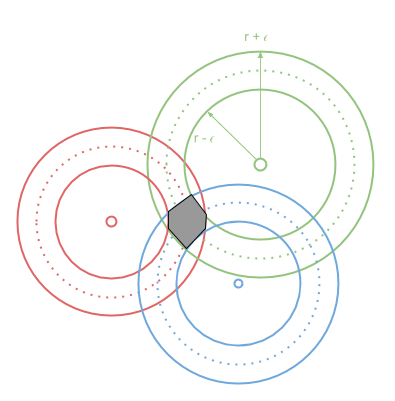
\includegraphics[scale=0.6]{cellbased}
  \caption{\emph{Cellbased} - área de intersecção(Fonte: autores)}
\end{figure}
\FloatBarrier

O ponto sensível dessa linha de pensamento é o fato que, devido às possíveis variâncias no erro, em alguns casos pode ocorrer o ilustrado abaixo, em que a área alvo não se fecha como deveria. Para estes casos é necessário tratamento especial, ou tentando inferir valores mais adequados por proximidade entre os pontos de intersecção par-a-par das circunferências ou simplesmente tomando-os como dados inválidos demais e descartando-os.

\begin{figure}[ht]
  \centering
    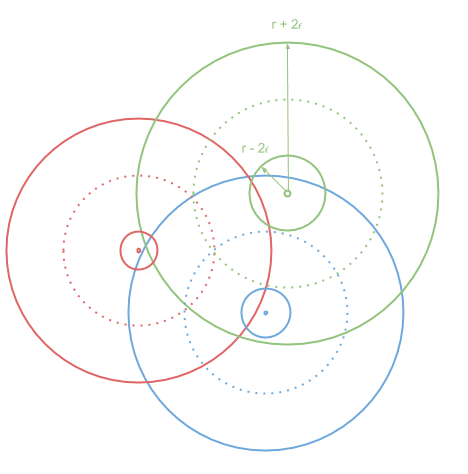
\includegraphics[scale=0.7]{cellbased-offrange}
  \caption{\emph{Cellbased} - área de intersecção fora do alcance (Fonte: autores)}
\end{figure}
\FloatBarrier


\chapter{Metodologia do Trabalho}
Seguindo as orientações de projeto de embarcados indicadas pelo professor orientador \cite{apostilaSE}, inicialmente é necessário levantar e descrever os requisitos funcionais e não funcionais do sistema - o que é feito já no capítulo seguinte.

A segunda etapa consiste na definição da arquitetura do projeto, para qual os possíveis componentes são associados estabelecendo uma composição que cubra os requisitos funcionais do projeto. A arquitetura é descrita no capítulo 6.

A seguir, aos componentes visíveis no plano físico, o que é feito no capítulo 5. Por fim, é implementado a arquitetura que foi projetada.

É adotada metodologia top-down visto que primeiro é definido o produto que se deseja obter para poder segmentar as tarefas a serem realizadas em micro serviços.

Ao mesmo tempo o projeto utiliza duas abordagens. Em alguns aspectos é utilizado o modelo em cascata, pois, por se tratar de um trabalho de formatura, é natural que algumas otimizações sejam reservadas para projetos futuros. Por esse ponto de vista, é como se cada projeto fosse uma curva na espiral.

Por outro lado, dada a abrangência tecnológica do projeto, em frentes como a interface será adotado o modelo espiral, pois neste caso modificações eventuais são menos custosas em tempo e orçamento. Portanto, estão planejados testes de usabilidade do \emph{software} em diversas etapas de produção.


\chapter{Especificação de Requisitos de Sistema}
O funcionamento essencial do sistema, o que define seus requisitos funcionais, requer que a posição dos macacos seja possível de ser medida, armazenada e mostrada para o usuário.

Além desses, são levantados os requisitos não funcionais, que trabalham aspectos necessários e complementares para o bom funcionamento do sistema, muitas vezes previstos pelo público solicitante do mesmo.

No SIMIOS, os principais requisitos não funcionais foram apontados por pesquisadores biólogos e veterinários com experiência em monitoramento de macacos. Dentre eles, está que o peso da mochila que será anexada ao animal não deveria ultrapassar 10g para não influenciar em seu comportamento nem sobrecarregá-lo, visto que o principal grupo de foco (saguis) tem peso médio de 400g. Para isso, é interessante que todos os componentes da mochila sejam o mais leves possível.

Outra situação apontada é o fato de que toda vez que a bateria do aparelho tiver de ser trocada, o veterinário deverá capturar o macaco e sedá-lo, o que é bastante prejudicial para a confiança que o animal constrói pelo ser humano. Dessa forma, é desejável que a eficiência energética do dispositivo embarcado seja alta para que a bateria tenha de ser trocada com a menor frequência possível.

Além da mochila do animal, espera-se que os dados coletados sejam confiáveis. Isso envolve garantir a autenticidade e a ausência de erros, ou seja, que eles estejam sendo de fato enviados íntegros pelo macaco a quem estão associados. Assim, evita-se casos em que o dispositivo possa ter sido removido acidentalmente e, por exemplo, enroscado em uma árvore ou em que existam interferências ruidosas no sinal capazes de alterar significativamente as medições enviadas. Também é relevante que o acesso à informação seja possível somente para pessoas autorizadas, envolvendo conceitos como autenticação e codificação.

SIMIOS é um sistema que, estruturalmente, poderia ser contextualizado em praticamente qualquer aplicação que se tenha algo a ser rastreado, seja um ser vivo ou não, para qual a precisão do GPS seja insuficiente. Portanto, de maneira geral, também é interessante que o sistema tenha escalabilidade em todos os aspectos - que os dispositivos embarcados nos animais possuam sensores diversos e que, possivelmente, toda a aplicação suporte que uma quantidade maior de variáveis e de usuários seja inserida.

Por fim, é sempre relevante que a interface com o usuário siga princípios de Experiência de Usuário (\emph{User Experience} - UX), especialmente se considerando que uma quantidade grande de dados deve ser visualizada de forma intuitiva e simples por pesquisadores. Os princípios seguidos por este trabalho se basearam naqueles descrito por Preece, Sharp e Rogers em \cite{preece}. É fortemente desejável, mas não necessário, que a forma de apresentação dos dados se adeque ao domínio do problema de forma a facilitar o trabalho dos investigadores e acelerar a formatação dos dados.

\begin{figure}[ht]
  \centering
    \includegraphics[scale=0.7]{esquematico}
  \caption{Resumo gráfico do sistema (Fonte: autores)}
\end{figure}
\FloatBarrier


\chapter{Tecnologias Utilizadas}
Considerando os aspectos discutidos no capítulo 2 sobre possíveis e impossíveis instrumentos para o nosso contexto, por fim foram selecionadas as tecnologias que serão efetivamente utilizados no projeto, as quais são descritas neste capítulo.

\section{Dispositivos Embarcados}

Partindo-se deste requisito, selecionou-se a plataforma de desenvolvimento \emph{SensorTag} da \emph{Texas Instruments} como componente embarcado que ficará em cada macaco e nos pontos de acessos nas árvores. Trata-se de uma placa leve e comercialmente atraente, que contém 6 sensores, incluindo de temperatura, e Bluetooth de Baixo Consumo Energético (BLE - \emph{Bluetooth Low Energy}) ou Sub-1GHz. Seu \emph{datasheet} pode ser encontrado nas referências deste trabalho \cite{datasheet}.

Além do \emph{SensorTag}, foi selecionado um \emph{Raspberry Pi} 2 para receber os dados de uma placa \emph{SensorTag} central via Transmissor/Receptor Assíncrono Universal (UART - \emph{Universal Asynchronous Receiver/Transmitter}). Tal placa central deverá receber dados dos demais pontos de acesso, e estes dados serão armazenados em um servidor pelo \emph{Raspberry Pi}.

\subsection{Sensortag}

\begin{figure}[ht]
  \centering
  \caption{Componentes do \emph{SensorTag}}
    \includegraphics[scale=0.5]{sensortag}
  \centerline{\small{Fonte: \emph{Texas Instruments}}}
\end{figure}

O código da placa dentre os produtos da TI é CC1350STK. Este é um dispositivo que é facilmente integrável com aplicações de tecnologia móvel (tendo inclusive um aplicativo aberto oficial da TI que pode ser baixado nas lojas de aplicativo e ser usado em conjunto com as placas).\\

A placa contém um microcontrolador que tem funcionalidades de comunicação sem fio, um processador principal \emph{ARM Cortex} M3 de 32 \emph{bits} com \emph{clock} de 48MHz e uma variedade de periféricos, como temporizadores de propósito geral, conversor analógico-digital, pinos de propósito geral, entre outros.

\section{Servidor}
Foi escolhido o banco de dados relacional \emph{MySQL} da \emph{Oracle} por se tratar de um sistema de código aberto simples, embora completo.

O projeto SIMIOS prevê o rastreio de animais em reservas, o que envolve, como visto anteriormente, no máximo cerca de 10 animais em grandes reservas. Dessa forma, sabemos que não envolve sobrecarga de acessos por segundo e mesmo isto poderia ser corrigido com \emph{buffering}.

Um ponto negativo do \emph{MySQL} é que sua escalabilidade pode ser prejudicada - cada servidor tem um tamanho limitado e cada conjunto de dados só pode ser alocado em um servidor (não suporta particionamento), o que pode ser prejudicial em casos que deseja-se guardar no banco grande quantidade de dados. Para corrigir tal empecilho é possível implementar importação de dados.

\section{Software}
Para desenvolvimento do programa computacional que é executado no servidor, foi escolhida a linguagem de programação \emph{Java}, com suporte de \emph{frameworks} \emph{Spring} e \emph{Java Persistence API} (JPA), facilitando principalmente os processos de queries do banco de dados, de autenticação e autorização e de mapeamento de interface \emph{model-view-controller} (MVC).

Por se tratar de uma aplicação de histórico de dados, pouquíssimo processamento está previsto e a computação pode ser realizada em tempo real pelo computador do usuário. Dessa forma, não se faz necessário o uso de linguagem de programação de execução eficiente (C++, por exemplo).


\include{projeto-implementacao}

\chapter{Testes e avaliação}

Foi determinada fundamentalmente a necessidade de avaliação do sistema sob duas frentes principais: consumo energético e precisão da posição obtida. 

Para tanto, foi elaborado teste para a determinação da precisão na medida da distância entre o ponto de acesso e o target. Dada a constante de propagação determinada como 2,95 (ver apêndice 2), foram comparados os valores exibidos pelo ponto de acesso e os medidos por uma trena, os quais estão disponíveis na tabela a seguir.

\begin{table}[ht]
\centering
\caption{Distâncias medidas pelo AP e pela trena}
\vspace{0.5cm}
\begin{tabular}{l|cccccccc}
\hline
\makecell{Distâncias pela \\ trena (m)} & 0,5 & 1,0 & 2,0 & 3,0 & 4,0 & 5,0 & 6,0 & 7,0 \vspace{0.4cm}\\

\makecell{Distâncias \\ pelo AP (m)} &
\makecell{0,79 \\ 0,86 \\ 0,73 \\ 0,86 \\ 0,63 \\ 0,63 \\ 0,63 \\ 0,63 \\ 0,63 \\ 0,63 \\ 0,63} &
\makecell{1,00 \\ 1,08 \\ 1,08 \\ 1,00 \\ 1,00 \\ 1,00 \\ 1,08 \\ 0,68 \\ 1,26 \\ 1,00 \\ 1,00} &
\makecell{0,73 \\ 0,73 \\ 0,73 \\ 0,86 \\ 1,37 \\ 1,87 \\ 1,60 \\ 1,50 \\ 1,48 \\ 1,37 \\ 1,48} &
\makecell{8,22 \\ 2,76 \\ 3,22 \\ 2,55 \\ 2,18 \\ 2,18 \\ 2,18 \\ 2,02 \\ 2,18 \\ 2,55 \\ 1,60} &
\makecell{2,15 \\ 1,82 \\ 2,78 \\ 2,56 \\ 2,78 \\ 2,35 \\ 2,56 \\ 3,30 \\ 3,03 \\ 2,78 \\ 2,56} &
\makecell{3,59 \\ 2,56 \\ 4,26 \\ 3,03 \\ 3,91 \\ 8,43 \\ 7,74 \\ 5,05 \\ 6,53 \\ 5,05 \\ 6,53} &
\makecell{4,64 \\ 4,64 \\ 4,64 \\ 3,91 \\ 3,03 \\ 2,56 \\ 2,56 \\ 5,99 \\ 4,26 \\ 14,07 \\ 7,11} &
\makecell{7,04 \\ 5,15 \\ 6,51 \\ 10,40 \\ 7,61 \\ 13,14 \\ 8,90 \\ 3,77 \\ 4,08 \\ 2,98 \\ 4,76}
\vspace{0.4cm}\\

\makecell{Distância média \\ pelo AP (m)} & 0,69 & 1,02 & 1,24 & 2,88 & 2,61 & 5,15 & 5,22 & 6,76
\end{tabular}
\end{table}

\begin{table}[ht]
\centering
\caption{Erro quadrático médio e máximo para cada n}
\vspace{0.5cm}
\begin{tabular}{l|c}
\hline
Erro quadrático médio (m) & 1,52 \vspace{0.4cm}\\
Erro quadrático máximo (m) & 3,04
\end{tabular}
\end{table}

Dessa forma, foi possível determinar o erro quadrático obtido, para o qual conclui-se que o sistema apresenta erro médio razoavelmente preciso, embora ainda alto se comparado ao erro do GPS, mas que pode chegar até 3 metros, que, para uma escala baixa como a de até 7 metros é bastante alto. 

\begin{figure}[ht]
  \centering
    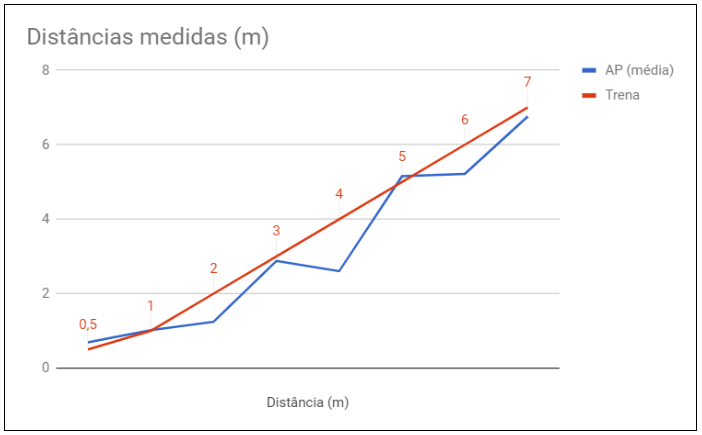
\includegraphics[scale=0.79]{graph-test-dist}
  \caption{Gráfico das distâncias medidas (Fonte: autores)}
\end{figure}

\begin{figure}[ht]
  \centering
    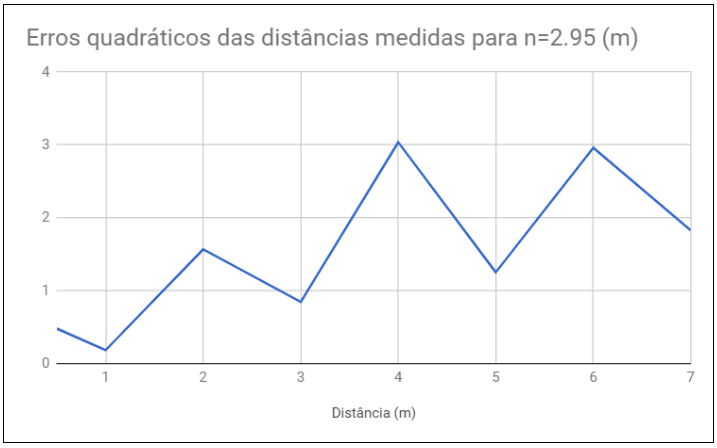
\includegraphics[scale=0.79]{graph-test-erro}
  \caption{Gráfico do erro quadrático para as distâncias medidas em n=2.95 (Fonte: autores)}
\end{figure}

No que se refere ao consumo energético, o único teste prático que foi pensado exigiria expor uma bateria nova à exaustão e calcular o tempo tomado. No entanto, como dimensionamos o sistema para que possa durar semanas, este teste é pouco praticável e fica dentro do escopo secundário do projeto.


\chapter{Considerações Finais}

\section{Conclusões do Projeto de Formatura}
O presente projeto é composto por módulos bastante distintos e elaborados em diversos níveis de abstração: apresentando considerações acerca do \emph{hardware} e \emph{firmware} de placas a serem utilizadas até a elaboração do \emph{software} de uma aplicação \emph{web} de alto nível.

Contudo, todos os objetivos principais propostos que formam o cerne da funcionalidade: de obter informações acerca do animais de forma constante, de armazenar essas informações para partes interessadas e de apresentá-las de forma clara; foram atendidos pela presente implementação. O primeiro se correspondeu pela interação entre o módulo aplicado aos macacos e aquele aplicado às árvores que mantém contínua vigília sobre os animais enviando informações sobre sua localização. O segundo se alcançou na construção de um banco de dados contendo todos os dados observados de onde o sistema for instalado, cujo conteúdo disponibilizar-se-ia a quaisquer pesquisadores interessados para análise dos dados. O último se concretiza na disponibilidade dos dados em forma de mapas ou tabelas, como for mais proveitoso, através de uma aplicação \emph{web}.

Em relação aos requisitos não funcionais levantados, destaca-se o cumprimento da exigência de generalização em relação ao objeto de observação do sistema; de fato, apesar de destinado à aplicação em símios de pequeno porte, com pouca ou nenhuma alteração o sistema pode ser facilmente adaptável para qualquer outro animal de comportamento similar ou a objetos inanimados que se queira investigar. Isto se deve à confirmação de que toda a base do sistema até o nível do banco de dados não exige configuração de qualquer parâmetro relacionado aos animais ou ao seu ambiente. Conclui-se então que o sistema é genérico o bastante para diversas aplicações, mas ressalva-se a necessidade de adaptar as informações coletadas para o novo domínio do problema.

Por outro lado, alguns aspectos do trabalho ficaram aquém dos resultados esperados. Como exemplo pode-se expor o fato dos módulos a serem carregados pelos macacos não atenderem à especificação de peso determinada, constituindo mais do que 10g, impedindo a observação de símios de menor porte. Isso não inviabiliza a monitoração pretendida, visto que a posição dos macacos ainda é assimilada e a monitoração da maioria dos animais não se torna irrealizável.

Outro exemplo pode ser feito da escolha de utilizar um nó central para condensar as informações do módulos dos pontos de acesso no coletor que, em contrapartida, prejudica a escalabilidade do sistema já que demanda que todos os pontos de acesso estejam a distância de transmissão do nó central. É possível resolver este ponto adaptando o sistema para que seja usado um protocolo de Redes \emph{Mesh}, viabilizando a expansão da rede.

Além disso, em sua presente iteração o sistema não usufrui do acoplamento de outros sensores embutidos no \emph{SensorTag} como foi planejado, já que o foco residia na aquisição de informações sobre o posicionamento. Adaptações em todos os âmbitos do projeto devem ser feitas para possibilitar a captação e exibição de dados de outros sensores presentes na placa.

Dois pontos finais devem ser notados neste balanço. Primeiramente a dificuldade de instalação do sistema se mostrou uma questão complexa e imprevista em sua concepção. Tanto pela variação ambiental da constante necessária para calcular as distâncias a partir do RSSI de forma confiável, como pelas interferências no sinal e limites de distância aos quais a comunicação entre as placas estão sujeitas mostra-se que os requerimentos para o bom funcionamento do SIMIOS não são triviais. Isso apresenta dificuldade notável na implementação do sistema em reservas mais diversas ou próximas a ambientes urbanos, como é o caso do Instituto Butantan. Para tanto um estudo mais aprofundado da variação das constantes ao longo do espaço disponível e uma redundância maior na transmissão dos sinais seriam benéficos para o projeto.

Finalmente, não se deve ignorar os custos financeiros relacionados à possível implantação deste sistema em grande escala. É necessário considerar que para cada objeto de estudo é preciso adquirir uma placa \emph{SensorTag}, assim como para cada ponto de acesso nas árores, número que aumenta a cada incremento na área de observação. Além disso há custos marginais na ampliação do banco de dados e servidores, o que resulta em um gasto nada trivial na expansão do sistema. Não obstante, dadas as alternativas de tecnologias atualmente disponíveis, apresentadas no segundo capítulo deste documento, a implementação proposta ainda se revela a opção de menor custo orçamentário.

\section{Contribuições}

Com o cumprimeto das funcionalidades necessárias neste sistema, acredita-se que o mesmo há de impactar de forma positiva os trabalhos de pesquisa em reservas nas quais se venha a instalar. Foi com o benefício de profissionais acadêmicos e de saúde animal que se baseou a elaboração das linhas guia deste projeto.

Em virtude dos estudos sobre as tecnologias presentes e das informações obtidas diretamente de profissionais da área, é possível dizer que, em comparação com as opções disponíveis de monitoramento de animais no mercado, as funcionalidades do SIMIOS atendem mais veementemente as necessidades correntes de primatologistas. Portanto o sistema contribui com uma solução mais bem adaptada aos profissionais de saúde e de comportamentalismo animal dadas as necessidades apresentadas destes grupos.

Atualmente o potencial de pesquisa nos campos de estudo da monitoração de animais, tanto no que diz respeito a pesquisas biológicas, como veterinárias quanto na esfera da Saúde Única é pouco explorado. Logo também é de interesse dos autores, não só satisfazer os requisitos do presente projeto, mas também dar destaque para tal nicho. Espera-se então que este trabalho sirva como inspiração e/ou ponto de partida para outros que almejam objetivos próximos através de metodologias similares. Adiciona-se a isso a expectativa de contribuições futuras como alternativas ao próprio SIMIOS, seguindo ou não os mesmos paradigmas ou as mesmas metodologias.

Com isso em mente, pretende-se deixar, através deste trabalho, uma variedade de contribuições realizadas pelos autores para qualquer um que planeje realizar um projeto ou sistema semelhante ou deseje usufruir dos módulos, ferramentas ou técnicas aqui desenvolvidos. Dentre eles é possível destacar: a elaboração da arquitetura do projeto; a integração e adaptação dos projetos disponibilizados pela Texas Instruments para compor o \emph{Firmware} da placa \emph{SensorTag}; a composição de mensagens contendo as informações necessárias a serem transmitidas entre as placas \emph{SensorTag}, assim como sua transmissão, recepção e interpretação no módulo controlador; a implementação do módulo controlador, usando o \emph{Raspberry Pi} como \emph{Gateway}; a organização do banco de dados de forma conveniente para a aplicação; o método pelo qual é calculada a posição de um elemento de estudo a partir da sua distância dos pontos de acesso (algoritmo de Trilateração); e a maneira como são organizadas e disponibilizadas as informações colhidas em uma interface \emph{Web}.

\section{Perspectivas De Continuidade}

Dadas as expectativas não cumpridas do trabalho, as primeiras propostas de continuidade pretendem atendê-las. Primeiramente a escalabilidade do sistema pode ser melhorada com o uso de outras técnicas de comunicação, como redes \emph{Mesh}, na transmissão de dados entre módulos periféricos e pontos de acesso, permitindo uma configuração que consiga cobrir uma área maior. No mesmo âmbito, os sensores da placa podem ser configurados para enviar seus dados coletados juntamente com as mensagens sobre distância, com suporte nos módulos de envio e armazenamento é possível coletar uma gama maior de informações, limitada apenas à variedade de sensores na placa e ao tamanho máximo das mensagens transmitidas. Isso permitiria, por exemplo, a obtenção de informações sobre a temperatura de animais na região, uma das principais métricas no mapeamento da disseminação da febre amarela.

Para outros projetos que pretendem aproveitar os resultados deste, facilmente é possível adaptar o sistema para demais ambientes de uso, onde, além de problemas peculiares de cada ambiente, deve-se apenas atentar à determinação da constante eletromagnética do meio em questão e a eventuais desafios na transmissão de dados, como interferências comuns em comunicações sem fio. Além disso, a adaptação é igualmente fácil para outros objetos de estudo a serem observados, notando-se apenas que a mudança do domínio do problema pode acarretar mudanças em seus requisitos, necessitando, por exemplo, de continentes mais apropriados para as placas SensorTags considerando outras espécies de animais.

São propostas adicionais de grande proveito para a melhora no bom funcionamento do sistema: o aumento do paralelismo e uso de threads tanto nos módulos de ponto de acesso, para garantir que mais leituras possam ser feitas em um mesmo local, quanto no módulo coletor, para evitar que este se torne um gargalo da aplicação; e a realização de mais transmissões nas comunicações ou a exploração de mais componentes no protocolo para garantir a integridade das informações transmitidas, como o emprego de mensagem de \emph{callback}.

Outras melhorias viáveis tocam questões relacionadas à manipulação da quantidade massiva de dados medidos. Na entrevista, a prof$^a$. Dr$^a$. Cristiane Pizzutto aponta que deve lidar com os dados manualmente e que utilizam planilhas para obter estatísticas, portanto seria interessante pensar em injetar conceitos de \emph{Big Data} que corroborem com o processamento dos dados, assim como princípios de Experiência de Usuário (\emph{User Experience} - UX), para que a forma de apresentação dos dados se adeque ao domínio do problema de maneira a facilitar o trabalho dos investigadores e acelerar a formatação dos dados. Seguindo tal intenção de aprimorar a interação do usuário com a interface disponibilizada, foi realizada prototipação de uma possível aplicação móvel com emprego de Realidade Aumentada, cujo estudo está disponível no apêndice 5.

Por fim, se o compromisso entre fatores for reavaliado é possível dar sequência ao projeto utilizando outra tecnologia na obtenção da distância, como o uso de placas mais baratas, mas com menor variedade de sensores ou protocolos de comunicação. Dessa forma seria possível trocar a variedade de informações coletadas pela redução no custo. Ou contrariamente, pode-se adquirir placas mais caras, porém com alcance superior ou faixa de transmissão menos suscetível a falhas. Trocando neste caso um aumento no custo financeiro do projeto por uma precisão e confiabilidade maior dos dados. De qualquer forma que se pense refatorar o sistema, partes dele, como o banco de dados ou a aplicação web nos casos exemplificados, ainda podem ser, e recomenda-se que sejam, reaproveitadas.


% ========== Referências ==========
% --- IEEE ---
%	http://www.ctan.org/tex-archive/macros/latex/contrib/IEEEtran
%\bibliographystyle{IEEEbib}

% --- ABNT (requer ABNTeX 2) ---
%	http://www.ctan.org/tex-archive/macros/latex/contrib/abntex2
\bibliographystyle{abntex2-num}

\bibliography{bibliography.tex}


% ========== Apêndices (opcional) ==========
\apendice
\include{apendice1}
\chapter{Determinação da constante de propagação}

A constante de propagação do ambiente determinada pela TI deve ser definida empiricamente. Portanto, foram tomados dez valores RSSI para distâncias conhecidas, medidas com uma trena, para que pudessem ser verificados os pontos críticos em que pudéssemos nos manter dentro do erro previsto. Além disso, foi medido RSSI consistente de -60 dB para 1 metro de distância.

\begin{table}[ht]
\centering
\caption{Intensidades observadas para cada distância medida com trena}
\vspace{0.5cm}
\begin{tabular}{l|ccccccc}
\hline
Distância (m) & 0,5 & 1,7 & 2,5 & 5 & 7,5 & 10 & 12,5 \vspace{0.4cm}\\

RSSI (dB) &
\makecell{-56 \\ -57 \\ -62 \\ -56 \\ -55 \\ -58 \\ -61 \\ -62 \\ -63 \\ -63 \\ -63 \\ -63 \\ -63} &
\makecell{-69 \\ -63 \\ -63 \\ -64 \\ -64 \\ -65 \\ -69 \\ -69 \\ -69 \\ -69 \\ -69 \\ -69 \\ -65} &
\makecell{-72 \\ -69 \\ -62 \\ -62 \\ -71 \\ -70 \\ -64 \\ -63 \\ -64 \\ -63 \\ -64 \\ -63 \\ -62} &
\makecell{-86 \\ -79 \\ -77 \\ -79 \\ -81 \\ -82 \\ -82 \\ -81 \\ -81 \\ -80 \\ -80 \\ -81 \\ -81} &
\makecell{-85 \\ -90 \\ -86 \\ -85 \\ -84 \\ -84 \\ -85 \\ -90 \\ -91 \\ -90 \\ -87 \\ -87 \\ -86} &
\makecell{-81 \\ -81 \\ -82 \\ -82 \\ -81 \\ -82 \\ -84 \\ -84 \\ -85 \\ -84 \\ -85 \\ -87 \\ -86} &
\makecell{-84 \\ -89 \\ -96 \\ -96 \\ -90 \\ -93 \\ -90 \\ -95 \\ -95 \\ -94 \\ -98 \\ -96 \\ -97}
\vspace{0.4cm}\\

RSSI médio (dB) & -60,15 & -66,69 & -65,30 & -80,77 & -86,92 & -83,38 & -93,30
\vspace{0.4cm}\\

n & -0,05 & 2,90 & 1,33 & 2,97 & 3,08 & 2,34 & 3,04
\end{tabular}
\end{table}

Assim, tomando o RSSI médio para cada distância, são listados os coeficientes de propagação ideais de cada medida. Tomando a moda de aproximadamente 2,95 e a média de 2,6, foram calculadas as distâncias que seriam medidas para ambos os coeficientes e, então, calculado o erro quadrático em cada ponto.

\begin{figure}[ht]
  \centering
    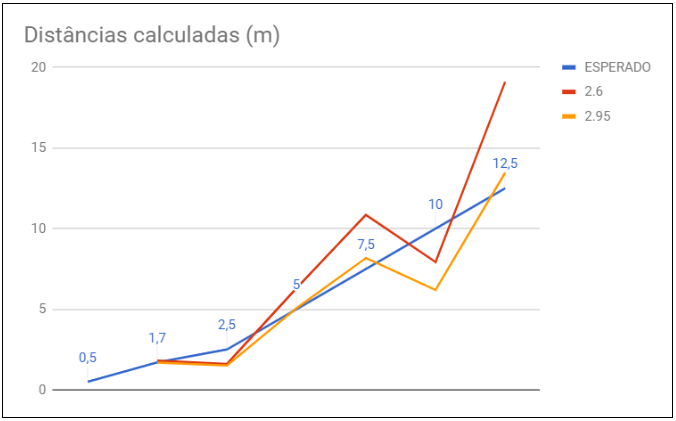
\includegraphics[scale=0.916]{graph-dist}
  \caption{Gráfico das distâncias calculadas para cada n (Fonte: autores)}
\end{figure}

\begin{figure}[ht]
  \centering
    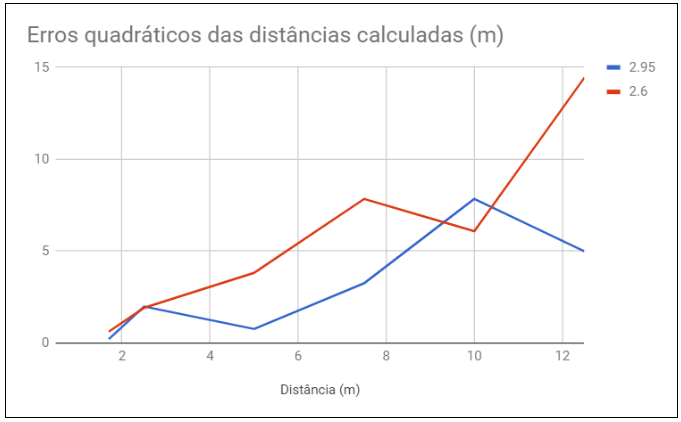
\includegraphics[scale=0.92]{graph-erro}
  \caption{Gráfico do erro quadrático para cada n (Fonte: autores)}
\end{figure}

\begin{table}[ht]
\centering
\caption{Erro quadrático médio e máximo para cada n}
\vspace{0.5cm}
\begin{tabular}{l|cc}
\hline
n & 2,95 & 2,6 \vspace{0.4cm}\\
Erro quadrático médio (m) & 2,82 & 4,06 \vspace{0.4cm}\\
Erro quadrático máximo (m) & 7,84 & 7,84
\end{tabular}
\end{table}

Por fim, concordou-se em utilizar o valor de n=2,95 por apresentar menor erro.

O processo realizado para a determinação do coeficiente de propagação poderia ser automatizado com algoritmos que inclusive considerassem mais valores caso fosse interessante expandir a aplicação dessa forma, por exemplo, anexando sonares aos pontos de acesso.

\chapter{Fluxo de telas da aplicação}

\begin{figure}[ht]
  \centering
    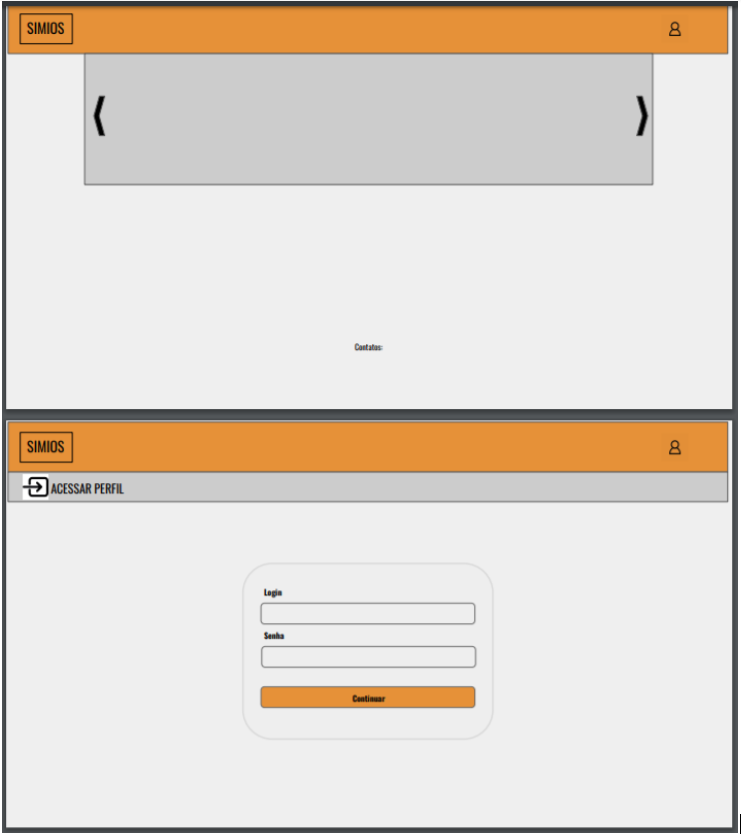
\includegraphics[scale=0.9]{fluxo-telas-1}
  \caption{Protótipo da homepage não autenticada e tela de login (Fonte: autores)}
\end{figure}

\begin{figure}[ht]
  \centering
    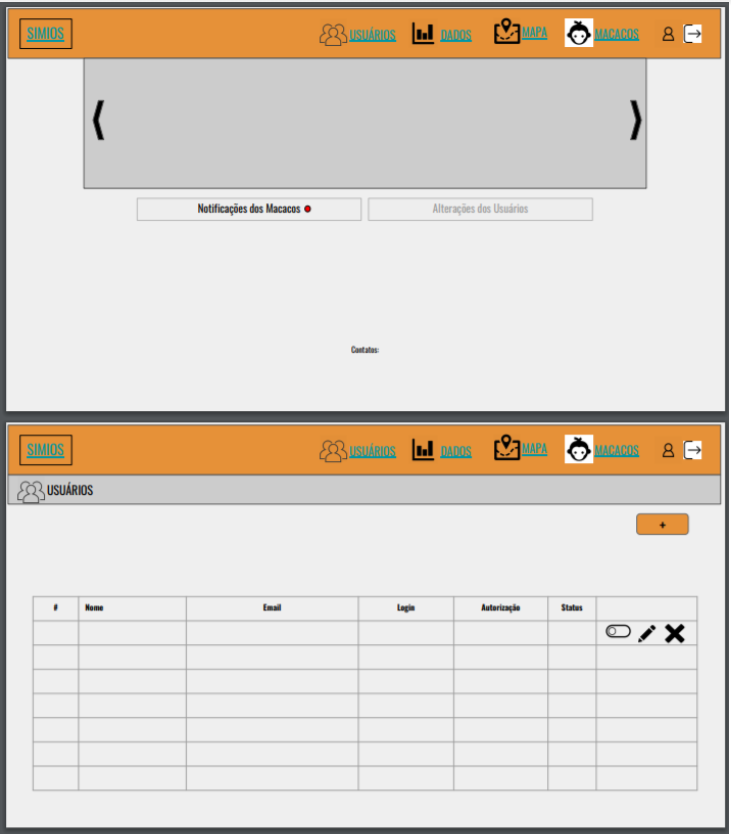
\includegraphics[scale=0.9]{fluxo-telas-2}
  \caption{Protótipo da homepage autenticada e da tela de listagem de usuários (Fonte: autores)}
\end{figure}

\begin{figure}[ht]
  \centering
    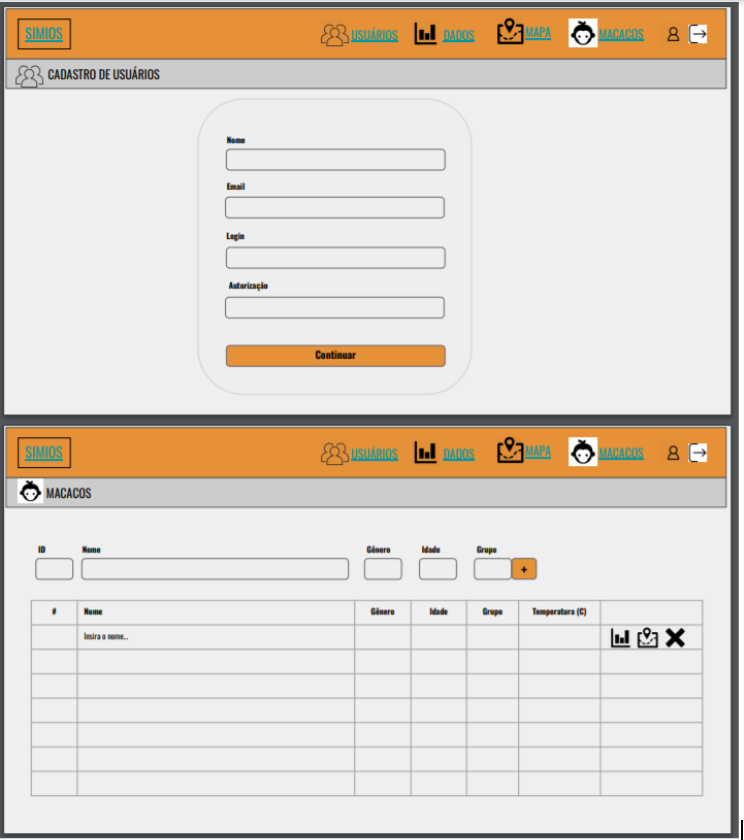
\includegraphics[scale=0.9]{fluxo-telas-3}
  \caption{Protótipo das tela de cadastro de usuários e listagem de símios (Fonte: autores)}
\end{figure}

\begin{figure}[ht]
  \centering
    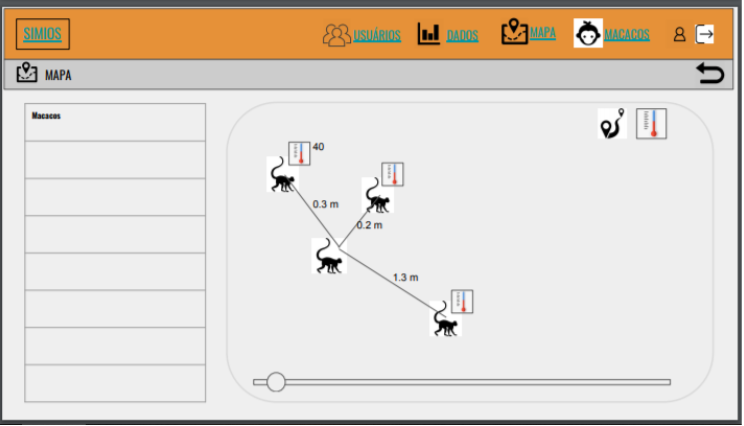
\includegraphics[scale=0.9]{fluxo-telas-4}
  \caption{Protótipo da tela do mapa (Fonte: autores)}
\end{figure}


% ========== Anexos (opcional) ==========
%\anexo
%\chapter{Alpha}
%\chapter{}



\end{document}
